% Created 2024-10-18 Fri 12:26
% Intended LaTeX compiler: pdflatex
\documentclass[11pt]{article}
\usepackage[utf8]{inputenc}
\usepackage[T1]{fontenc}
\usepackage{graphicx}
\usepackage{longtable}
\usepackage{wrapfig}
\usepackage{rotating}
\usepackage[normalem]{ulem}
\usepackage{amsmath}
\usepackage{amssymb}
\usepackage{capt-of}
\usepackage{hyperref}
\usepackage{parskip,darkmode}
\enabledarkmode
\usepackage{tikz}
\usetikzlibrary{arrows, positioning}
\usepackage{booktabs,colortbl}
\usepackage{algorithm,algpseudocode}
\author{Arnav Gupta}
\date{\today}
\title{Inference And Planning}
\hypersetup{
 pdfauthor={Arnav Gupta},
 pdftitle={Inference And Planning},
 pdfkeywords={},
 pdfsubject={},
 pdfcreator={Emacs 29.4 (Org mode 9.7.11)}, 
 pdflang={English}}
\begin{document}

\maketitle
\tableofcontents

\section{Problem Solving}
\label{sec:org4f4d5d0}
Two methods for solving problems:
\begin{itemize}
\item \textbf{procedural}
\begin{itemize}
\item devise an algorithm
\item program an algorithm
\item execute the program
\end{itemize}
\item \textbf{declarative}
\begin{itemize}
\item identify knowledge needed
\item encode the knowledge in a representation (knowledge base - KB)
\item use logical consequences of KB to solve the problem
\end{itemize}
\end{itemize}

A logic consists of \textbf{syntax}, \textbf{semantics}, and \textbf{proof procedure}.

\textbf{Proof}: a sequence of sentences derivable using an inference rule
\subsection{Logical Consequence}
\label{sec:org5819281}
For a set of \textbf{statements} \(\{X\}\):
\begin{itemize}
\item a set of truth assignments is an \textbf{interpretation}
\item an interpretation that makes it true is a \textbf{model}
\item if it has no model, it is \textbf{inconsistent}
\end{itemize}

A statement is a \textbf{logical consequence} of a set of statements if the statement is true in every
model of the set.

\begin{table}[h]
    \centering
    \begin{tabular}{ccccccc}
        \toprule
        \( P \) & \( H \) & \( C \) & \( P \to(\neg H \to C) \) & \( P \to \neg H \) & \( P \to C \) \\
        \midrule
        \rowcolor{green!30!black!70}
        F & F & F & T & T & T \\
        \rowcolor{green!30!black!70}
        F & F & T & T & T & T \\
        \rowcolor{green!30!black!70}
        F & T & F & T & T & T \\
        \rowcolor{green!30!black!70}
        F & T & T & T & T & T \\
        T & F & F & T & F & F \\
        T & T & F & T & F & T \\
        T & T & T & T & F & T \\
        \rowcolor{green!30!black!70}
        T & F & T & T & T & T \\
        \bottomrule
    \end{tabular}
    \caption{Truth table with highlighted models, showing $P_{1}, P_{2} \models D$.}
\end{table}

An argument is \textbf{valid} if:
\begin{itemize}
\item conclusions are logical consequences of the premise
\item conclusions are true in every model of the premises
\end{itemize}
\section{Proofs}
\label{sec:orgeed1bc8}
\textbf{Knowledge Base}: set of axioms

KB \(\vdash g\) means \(g\) can be derived from KB using the proof procedure.
If it is true, then \(g\) is a theorem.

\textbf{Soundness}: if KB \(\vdash g\), then KB \(\models g\).

\textbf{Completeness}: if KB \(\models g\), then KB \(\vdash g\).

Assume a \textbf{closed world}:
\begin{itemize}
\item agent knows everything
\item if it cannot prove something, it must be false
\item negation is failure
\end{itemize}
\subsection{Bottom-Up Proof}
\label{sec:orgf4a3557}
\textbf{Forward chaining}: start from facts and use rules to generate all possible atoms

\begin{algorithm}
    \caption{Bottom-Up Proof}
    \begin{algorithmic}[1]
        \State $C \gets \{\}$  \Comment{Initialize the set of conclusions}
        \Repeat
            \State Select $r \in KB$ such that
            \State \quad $r$ is $h \gets b_1 \land \ldots \land b_m$
            \State \quad $b_i \in C \; \forall i$  \Comment{All premises are in $C$}
            \State \quad $h \notin C$  \Comment{$h$ is not already in $C$}
            \State $C \gets C \cup \{h\}$  \Comment{Add $h$ to the conclusions}
        \Until{no more clauses can be selected}
    \end{algorithmic}
\end{algorithm}

Forward chaining is sound and complete.
\subsection{Top-Down Proof}
\label{sec:orgcf188d8}
Start with query and work backwards, trying to see if it is proved from the premises.
\begin{algorithm}
    \caption{Top-Down Proof}
    \begin{algorithmic}[1]
        \Procedure{solve}{$q_1 \land \ldots \land q_k$}
            \State $ac \gets \text{"yes} \gets q_1 \land \ldots \land q_k$"  \Comment{Initialize the answer condition}
            \Repeat
                \State Select a conjunct $q_i$ from the body of $ac$
                \State Choose a clause $C$ from $KB$ with $q_i$ as the head
                \State Replace $q_i$ in the body of $ac$ by the body of $C$
            \Until{$ac$ is an answer}
        \EndProcedure
    \end{algorithmic}
\end{algorithm}

In the \uline{select} step, some selections will lead to solutions more quickly, though any should lead
to a solution in the end.
In the \uline{choose} step, if one choice doesn't give a solution, others may, so all must be tried.

KB can contain \textbf{relations} (predicates) or \textbf{quantification}.
\section{Planning and Actions}
\label{sec:orgc820c68}
\textbf{Planning}: decide what to do based on the agent's ability, goals, and state of the world; basically find
a sequence of actions to the goal

Assume:
\begin{itemize}
\item a single agent
\item deterministic world
\item no events outside the agent's control that change the state of the world
\item agent knows what state the world is in (full observability)
\item time progresses discreetly
\item goals are predicates of states that must be achieved/maintained
\end{itemize}

\textbf{Action}: partial function (some actions only possible from some states) from states to states

\textbf{Preconditions} of an action specify if it can occur. \textbf{Effect} of an action specifies resulting state.

\textbf{Causal rules} specify when a feature gets a new value. \textbf{Frame rules} specify when the feature keeps
its values.

In planning, the givens are:
\begin{itemize}
\item description of effects and preconditions of actions
\item description of initial state
\item goal to achieve
\end{itemize}

Achieved by finding a sequence of possible actions that will result is state that satisfies the goal.
\subsection{Forward Planning}
\label{sec:org25c200a}
Search in the state-space graph:
\begin{itemize}
\item nodes represent states
\item arcs correspond to actions legal from that state
\item plan is a path from the initial state to a goal state
\item heuristics can be important
\end{itemize}

\begin{center}
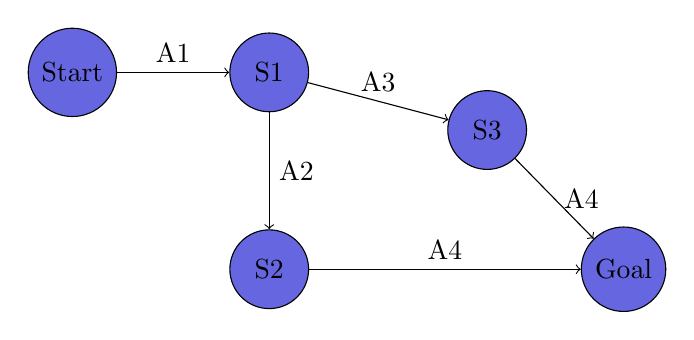
\begin{tikzpicture}[
    node distance=2.5cm,
    state/.style={draw, circle, fill=blue!80!black!60, minimum size=1cm}
]

    % Define state nodes
    \node[state] (start) {Start};
    \node[state] (s1) [right of=start] {S1};
    \node[state] (s2) [below of=s1] {S2};
    \node[state] (goal) [right of=s2, xshift=2cm] {Goal}; % Goal positioned to the right
    \node[state] (s3) [above right of=s2, xshift=1cm] {S3}; % Positioned above the edge

    % Draw edges between state nodes with action labels
    \path[->]
        (start) edge node[midway, above] {A1} (s1)
        (s1) edge node[midway, right] {A2} (s2)
        (s1) edge node[midway, above] {A3} (s3)
        (s2) edge node[midway, above] {A4} (goal)
        (s3) edge node[midway, right] {A4} (goal);
\end{tikzpicture}
\end{center}
\subsection{Regression Planning}
\label{sec:orgcb7a583}
Search backwards from the goal description with nodes corresponding to subgoals and arcs to actions:
\begin{itemize}
\item nodes are propositions (assignments of values to features)
\item arcs correspond to actions that can achieve goals
\item neighbours of a node specify what must be true immediately before the arc so that the node is true
immediately after
\item start node is the goal to be achieved
\item \(\text{goal}(N)\) is true if \(N\) is a proposition true of the initial state
\end{itemize}
\end{document}
